\section{Experimental Results \label{ExperimentalResults} }
This section summarizes the appendix to this project and the pipeline's development. The corresponding file for the appendix can be found under \path{ss20_lanz_2d_obstacle_avoidance/doc/thesis/Thesis_appendix.pdf}. The appendix lists all models trained as batches, where each batch contains models trained on a specific environment or with different parameters. Except for the pipeline's parameters, the appendix additionally lists results from the model's training and testing.\\

To guarantee a robust and successful process, suggestions from \cite{Goodfellow-et-al-2016} and \cite{DBLP:journals/corr/abs-1803-09820} are applied, as  discussed in \secref{monitoring}.  
One suggestion, which could be implemented directly, is to set up a functioning pipeline very early in the process to immediately discover and adjust functions or parameters, which cause errors or poor training performance. Even if one of the essential techniques to increase performance is to increase training data, the methods mentioned above were fundamental to acquire further knowledge about the model itself and the entire pipeline's execution. The training on small datasets to test the model's fitting ability, the recognition of duplicates at Feature Extraction or the correct prediction of images without obstacles are just a few examples where the techniques mentioned have been applied. The calculation of the Area Under the Curve and the visualization techniques gave a compelling insight into the model's performance, in a very exact and accurate in the former, and very intuitive, but extremely helpful in the latter.\\


The following subsection first gives a brief review of the pipeline development challenges and results and then discusses the pretraining and training phase. The first five batches trained are part of the pretraining phase, while the last batch, with knowledge applied from the pretraining, contains the final experimental results.

\subsection{Pipeline \label{pipeline}}
This section is about challenges faced while setting up the pipeline, during the early stages of the training process.\\

\textbf{Environment} As one of the requirements is to provide system independency, the project proposes a docker environment. A TensorFlow base image was chosen and extended with a ROS and TIAGo environment. As an interpreter, Python3 was used throughout the entire environment, which led to some ROS conflicts to solve. Using Python3 was rewarding in the end, as many libraries for machine learning like Scipy, Numpy, or Keras, could be used with up-to-date versions. Another challenge was to activate a graphical user interface within the docker environment for simulations, heatmaps, or graphs to be displayed or saved, or the implementation of functioning GPU support based on Tensorflow. Overall, it was very challenging, but rewarding to have all tools working and adjusted adequately for one environment.\\

\textbf{Data Acquisition} Setting up a robust and reliable Data Acquisition Controller was one of the most time-intense tasks for this project. During the entire process, functions had to be adjusted, rewritten, or extended to increase and guarantee a fully autonomous and safe data collection from different environments.\\

\textbf{Feature Extraction} As part of the concept is provided by \cite{nava2019learning}, the contribution for this part was mostly the proper implementation concerning the environment, architecture, and sensors used. Even if the concept was partially available, the effort to incorporate this stage within the pipeline was substantial. Additional functionalities, like error recognition mechanisms, a fully autonomous workflow, or the implementation of centralized parameter control, are among several extensions applied to this stage.\\

\textbf{Training} As well as for Feature Extraction, \cite{nava2019learning} provides a rough layout of the architecture setup with training scripts for datasets provided by the previous stage. As in Feature Extraction, the main challenge was the proper incorporation within the pipeline, with several new features and extensions applied as error recognition, autonomous workflow, file administration, and centralized parameter control.\\

\textbf{Performance Monitoring and Testing} To properly monitor the pipeline and have it run fully autonomous, several implementations were set up and iteratively adjusted, rewritten, or replaced. One complete replacement was the File Administration Class, which was considered too heavy and difficult to maintain after being used at the early stages. A subsequent version was created, easier to maintain, and use. It seemed practical to have a File Administration, logically store, name, and check files for consistency from the early stages upon, to save manual effort and time. Another handy tool was to implement custom error messages through all stages. This functionality was a beneficial debugging mechanism and provided useful hints of where changes had to be adapted. The visualization techniques in the form of videos and heatmaps were also beneficial to quantify a model's performance. It is much easier to look at a heatmap, instead of an array, and act upon its behavior. The entire manual testing, as described in \secref{sim_prototype}, could be done very effectively with heatmaps, representing predictions in real-time. Manual testing, compared with the Area under The Curve, could get additional insight into the model's behavior and performance.

\subsection{Pretraining and Debugging \label{pretraining}}

\textbf{Batch 1}\\
As in the chapter  11.3 of \cite{Goodfellow-et-al-2016}, which is about determining whether to gather more data or not, the author claims that if the validation set's performance is much worse than the training set's performance, the most effective way to increase a models performance is to gather more data for training. This concept can be observed in the first three models of Batch 1, which use a relatively small amount of input data. A more considerable amount of input returns better results for subsequent models on the validation set.\\

Another observation on Batch 1 is that most model's outer ranges, as $R_{1}$ or $R_{5}$, have inferior performance. As the outer range's performance is much lower overall models of Batch 1, in comparison to the center ranges, it appears reasonable to adjust parameters as the $laser range $, the $laser threshold$ or $safe_{d}$. Especially $safe_{d}$, which is a safe distance and determines the closest possible position the robot can approach an obstacle, impacts the gap of results among the center and outer ranges, as it directly influences how frequent the outer ranges are used. \figref{safe_d_adjustment} describes this concept, where a smaller value for $safe_{d}$ increases the use of the outer ranges.\\

A surprising result is delivered for Model 13 from Batch 1. The model's quality decreases over the quality of model 5, although a much more considerable amount of images is provided for training.\\

The learning rate for all models, except Model 14 and 15, is kept at 0.0002. As suggested by \cite{DBLP:journals/corr/abs-1803-09820}, and discussed in \secref{hyperparameters}, the learning rate can be increased if a model underfits. This concept is applied for Dataset 13 with the results of Model 14, which seems to be more stable at the validation loss. A further increase in the learning rate on the same dataset drastically decreased performance. This can be seen at the results of Model 15 and at \figref{learning_rate_test}.\\

The recognition of unknown obstacles performs poorly over the entire batch. Especially distances are not interpreted correctly. Ranges, on the other hand, are correctly predicted in some cases.\\

Distance accuracy also performs relatively low. It can be observed that with increasing distances of obstacles, their prediction gets more accurate. This behavior seems to be an issue of the parameter $laserthreshold$ and $safe_{d}$, which are adjusted on future batches.

\vspace{0.2 cm}
\begin{figure}[h]%[htbp]
\centering
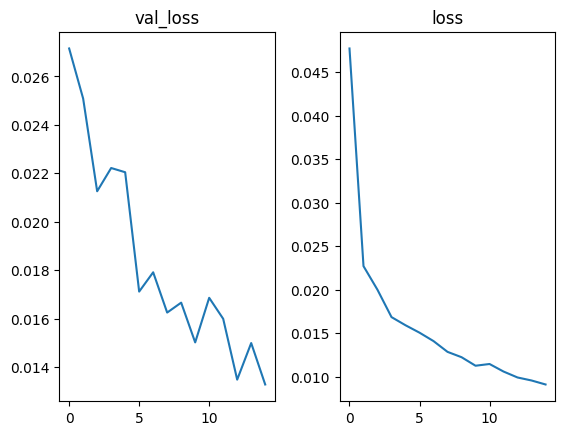
\includegraphics[width=0.30\textwidth]{3_models/models_13/graph_13.png}
\hspace{0.2 cm}
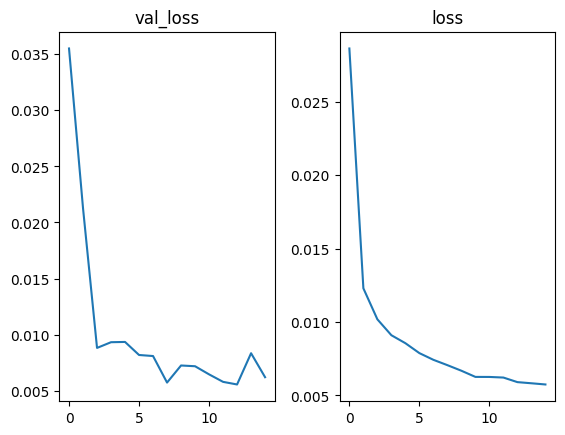
\includegraphics[width=0.30\textwidth]{3_models/models_14/graph_14.png}
\hspace{0.2 cm}
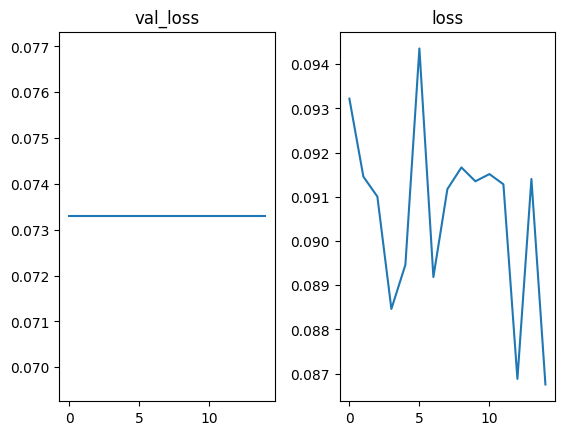
\includegraphics[width=0.30\textwidth]{3_models/models_15/graph_15.png}
\caption[]{Learning rate test with an increasing value run on three models. The last model's performance, drastically decreases.}
\label{learning_rate_test}
%\vspace{-50pt}
\end{figure}

Empty instances are recognized through all models except the last model of Batch 1. As the problem of not recognizing instances without obstacles has already been solved during debugging, this behavior is expected.\\

The correct recognition of ranges gradually increases with the number of images used. Model 5 provides the most accurate predictions of ranges for this batch.\\

Looking at the Area Under the Curve results, one might consider Model 4 as the winner for Batch 1. The reality is that Model 4 performs rather poorly on the simulation test for correct distances. The model seems to be too sensitive to see obstacles that are further away than the recording distance. As the Area Under the Curve is calculated on the validation set, it lacks the knowledge of obstacles further away than the recording distance, as all recordings on the validation set are within the recording distance range. Therefore, Model 5, instead of Model 4, is set as the winner for Batch 1. Model 5 is given a more considerable amount of training data, which reduces this too high sensitivity of Model 4, and allows it to generalize more efficiently.\\

\begin{figure}[H]%[htbp]
\centering
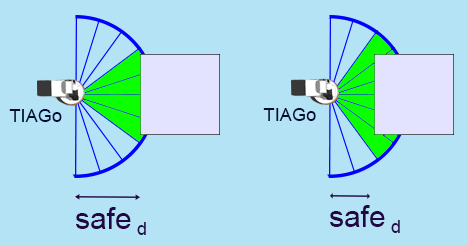
\includegraphics[width=1\textwidth]{Bilder/safe_d.png} 
\caption[]{Concept of the effect on ranges used by changing the parameter $safe_{d}$.}
\label{safe_d_adjustment}
\end{figure}


\textbf{Batch 2}\\
As this batch's environment provides a substantially more considerable variety of obstacles, the overall performance somewhat decreased compared to the results of Batch 1. As the average number of images extracted per obstacle decreases due to a greater variety, this behavior seems trivial. This side effect can be countered to increase the input as in Model 11, which provides the best results with 30000 images in the dataset. The greater variety has advantages as well when it comes to recognizing unknown obstacles, which also makes sense, as the probability of an unknown obstacle to be more similar to a known obstacle is higher if the variety is more significant, to begin with.\\

As the environment's complexity heavily increased, several adjustments are necessary to guarantee a robust and fully autonomous gathering of data. At the early stages, this environment caused the robot to get frequently stuck in a loop, which could be fixed by setting some timeouts if a particular state would not change.\\

\textbf{Batch 3}\\
To increase the side ranges performance, as discussed analyzing Batch 1, and in \figref{safe_d_adjustment}, the $laser threshold$ and  $safe_{d}$ are decreased for this batch. A low value like 0.2 for $safe_{d}$ causes collisions at certain angles of this environment's brick wall obstacle. The value can be set to 0.35 without the robot crashing.\\

The overall performance of high input models is satisfying but not perfect yet. It can be observed that the performance of the outer ranges averagely increased in comparison to Batch 1 or Batch 2. Especially Models 26, 27, and 28 provide pretty decent results. Also, the distance accuracy improves for the middle part, which is from 1 to 2 meters. For very close obstacles, the distance prediction is still not very accurate.\\

\textbf{Batch 4}\\
For this batch, the recording distance is changed. As the camera used for this simulation can recognize obstacles up to 8 meters, it might be rewarding to take advantage of that. As intermediary positions, a value of 81. This change increases the number of images recorded to about 154, for each bagfile. The increase of recording distance has several impacts. It requires a more considerable amount of computational resources, like the Neural Network's output instead of (1,155) for 31 intermediary positions increases to (1,405) for 81 intermediary positions. The time to create a dataset or train a model substantially increases.\\

A more considerable recording distance aims to make the model less sensitive to objects further away than the recording distance. This problem is discussed analyzing Model 4 at Batch 1.\\

While the first models' results are expected with respect to the rest of the pipeline results, the last model performs very poorly. Model 39 fails on all tests, like the Area Under the Curve, as well as on the manual simulation. More tests with more significant computational resources could probably be rewarding.\\

\textbf{Batch 5}\\
As some results of Batch 4 are shallow, and further analysis concludes that the cause might be an implementation error, the selection range, as well as the distribution of intermediary position is adjusted for this batch.\\ 

The selection range is a setting at Feature Extraction, which limits possible intermediary positions around a specific threshold or uses the entire bagfiles odometry information to find intermediary positions as described in \secref{finding_positions}.\\

The distribution of intermediary positions is a value which distributes the intermediary positions set over the recording distance. As the intermediary positions are set in decimeters, for a recording distance of 4 meters, 40 intermediary positions are chosen. If intermediary positions are applied as

\begin{equation}
\label{eqn:14} 
f(n) = \frac{n}{10}
\end{equation}

it would cause immense distances to get insufficient weight for training. The results can be seen at Batch 5, where all models have a deficient performance for distances starting at about 3.5 meters. For the final training, the denominator of the equation \ref{eqn:14} will be set higher. This change will shrink the intermediary positions within the recording distance and lead to more accuracy at distances that are further away.

\subsubsection{Conclusion Pretraining \label{conclusion_pretraining}}
The following main observations about the model's performances can be concluded from the pretraining phase. For each result, a proper solution is suggested and applied, to increase the model's performance further:

\begin{itemize}
\item Low results on the outer ranges over all batches
\item No distance recognition of unknown obstacles overall batches
\item Low performance of distance recognition, especially to distances in the immediate vicinity and the center of the prediction
\end{itemize}

\textbf{Outer ranges}\\
Increasing the results of the outer ranges is already discussed in the analysis of Batch 1. A decrease of the value $d_{safe}$ is suggested at this step. Another possibility is to increase the density of the environment. That change would lead to the outer ranges being used more frequently.\\

\textbf{Unknown obstacles}\\
Increasing the variety of obstacles would increase the probability of unknown obstacles to be recognized. 

\textbf{Distance recognition}\\
As the predictions for distances are unreliable overall batches, a sever calculation bug can be fixed after extensive analysis of the pipeline's results. The intermediary positions distribution parameters, over the recording distance, are adjusted, at Feature Extraction.\\

Interestingly, the performance issues mentioned are rather caused by calculation or implementation errors, instead of training parameters set wrong. This behavior can be concluded from the prediction being accurate for some models or some parts of the models. By some parts, a specific range or distance range is considered. The next chapter summarizes models trained, with knowledge and insight obtained from the pretraining phase.
\newpage

\subsection{Final Results \label{final_results}}
In this chapter, the final testing results are presented. Batch 6 is individually trained and contains seven models with images ranging from 2400 to 13840. Batch 6 can further be split into two sets of models, where the first set (Model 47, 48, 49, and 62) is trained on a recording distance of 4 meters, and the second set (Model 59, 60, and 61) is trained on a recording distance of 3.5 meters. As mentioned in \secref{conclusion_pretraining}, this batch is trained upon experience and knowledge gained from the pretraining phase.\\

By comparing the two sets, the overall performance is slightly better on the first. \figref{final_set_1} displays the gradual increase of Set 1, increasing the number of images from 3440 to 13840.

\begin{figure}[H]%[htbp]
\centering
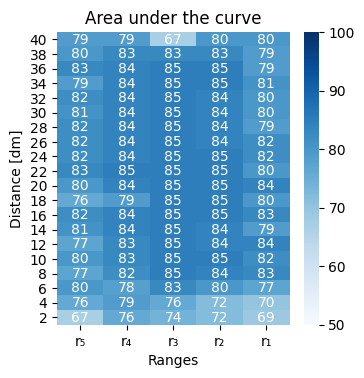
\includegraphics[width=0.31\textwidth]{4_plots/plots_47/AUC_47.png}
\hspace{0.2 cm}
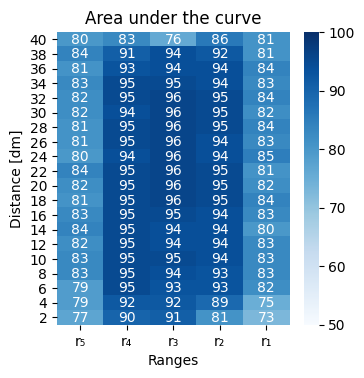
\includegraphics[width=0.31\textwidth]{4_plots/plots_48/AUC_48.png}
\hspace{0.2 cm}
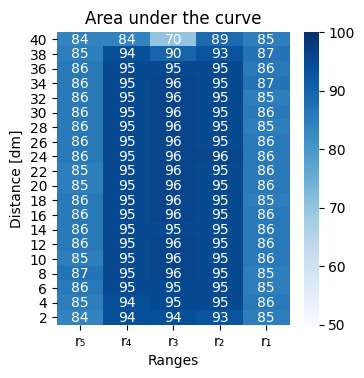
\includegraphics[width=0.31\textwidth]{4_plots/plots_49/AUC_49.png}
\caption[]{Comparsion of Model 47, 48 and 49, with a gradual increase of performance, relative to the increase of training data.}
\label{final_set_1}
\end{figure}

The following sub-chapter further compares the two best of all models. The manual testing results, which can be seen in the appendix in Table 6, show equally good results for both. Model 49 is further used to create a video displaying the results of its performance. The video can be obtained within the repository on the following path:
\path{ss20_lanz_2d_obstacle_avoidance/doc/thesis/Videos/Final_video.mkv} 

\subsubsection{Model 49 \label{model_49}}
One of the best of all models trained for this project is Model 49, which displays high accuracy on all tests. \figref{best_model_49} displays the Area under the Curve, the Training vs. the Validation loss, and a graph for the Generalization Error.\\

\textbf{AUC} The results of the Area under the Curve for Model 49 are among the best of all models trained. The outer, but especially the inner ranges, averagely display results up to 95. As the parameter $safe_{d}$ already had been at a minimal value, the model's outer range quality could be further increased by increasing the density of the environment as discussed in \secref{conclusion_pretraining}.\\

\textbf{Validation vs. Training loss} By looking at the second image of \figref{best_model_49}, the training loss is lightly lower than the validation loss, which indicates the model to be lightly overfitting. The validation loss, furthermore displays the desired horizontal line, as described in \cite{DBLP:journals/corr/abs-1803-09820}. This desired horizontal line can also be observed, looking at the results of Model 62 of Batch 6 in the appendix.\\

\textbf{Generalization Error} This plot is calculated by subtracting the training loss from the validation loss. The graph first increases and then stays in a horizontal form at around 0.01.

\begin{figure}[H]%[htbp]
\centering
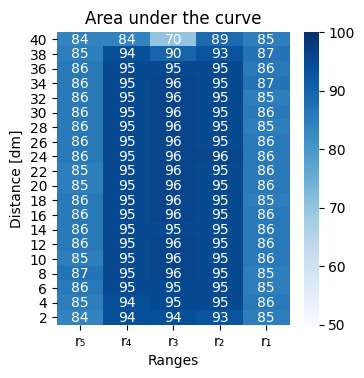
\includegraphics[width=3.8cm, height=4cm]{4_plots/plots_49/AUC_49.png}
\hspace{0.2 cm}
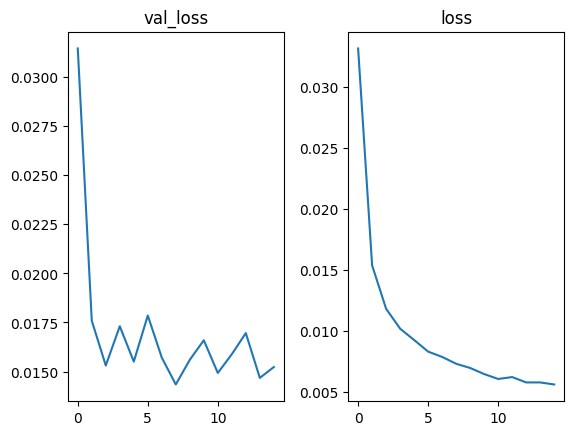
\includegraphics[width=4.8cm, height=4cm]{3_models/models_49/graph_49.png}
\hspace{0.2 cm}
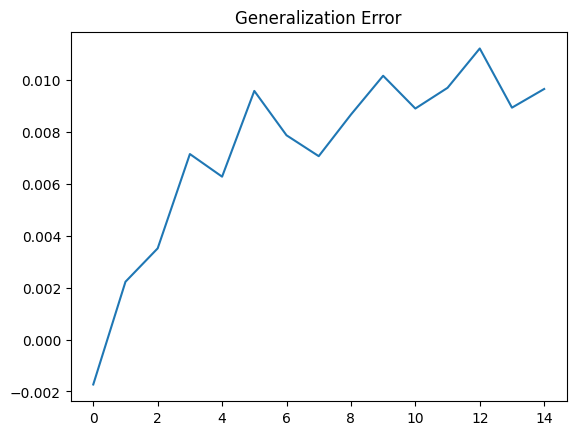
\includegraphics[width=4.8cm, height=4cm]{3_models/models_49/gen_loss_49.png}
\caption[]{Result plots for Model 49 of Batch 6.}
\label{best_model_49}
\end{figure}

\subsubsection{Model 62 \label{model_62}}
Another model worth mentioning is Model 62 of Batch 6. This model is trained on the same dataset as Model 49, with the difference of 30 epochs instead of 15 used.\\

\figref{best_model_62} displays the results of Model 62. While the results for the Area under the Curve nearly stays the same, the generalization error can be further decreased to about 0.004. This is due to a better performance of the validation loss, which fluctuates around 0.01. 

\begin{figure}[H]%[htbp]
\centering
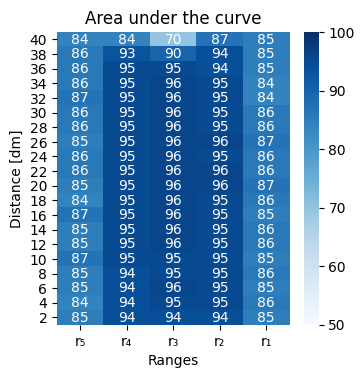
\includegraphics[width=3.8cm, height=4cm]{4_plots/plots_62/AUC_62.png}
\hspace{0.2 cm}
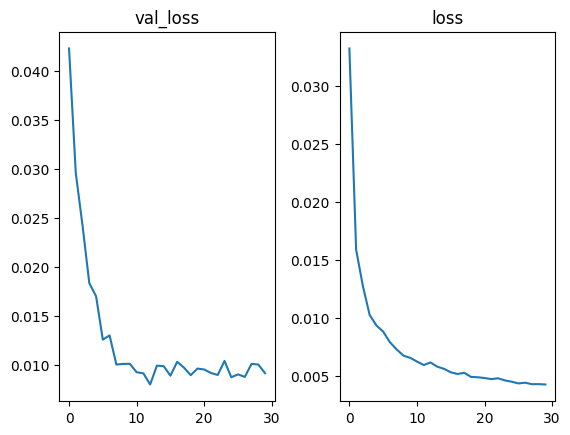
\includegraphics[width=4.8cm, height=4cm]{3_models/models_62/graph_62.png}
\hspace{0.2 cm}
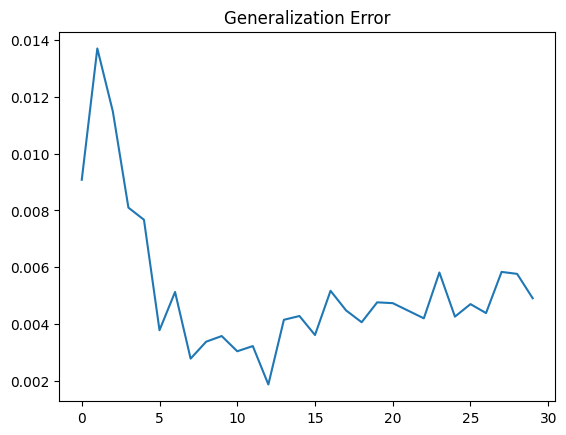
\includegraphics[width=4.8cm, height=4cm]{3_models/models_62/gen_loss_62.png}
\caption[]{Result plots for Model 62 of Batch 6.}
\label{best_model_62}
\end{figure}
